\documentclass[ms]{uncgdissertationexp2}

\usepackage{microtype, amsmath, amssymb, amsfonts, amsthm, graphicx, booktabs, syntax, subcaption, algorithm}
\usepackage[colorlinks=false]{hyperref}
\usepackage[noend]{algpseudocode}

\graphicspath{{img/}}

\chair{Stephen R. Tate}
\member{Chun Jiang Zhu}
\member{Insa R. Lawler}   

\student{Larry Joshua}{Crotts}
\title{Construction and Evaluation of a Gold Standard Syntax for Formal Logic Formulas and Systems}

%% Degree year.    
\degreeyear{2022}

\doublespacing

%% Theorem, Lemma, etc. environments.  You can rename if you wish.                    
% Theorem style and numbering convention                                              
\theoremstyle{plain}
\newtheorem{theorem}{Theorem}[chapter]
\newtheorem{lemma}[theorem]{Lemma}
\newtheorem{proposition}[theorem]{Proposition}
\newtheorem{conjecture}[theorem]{Conjecture}
\newtheorem{corollary}[theorem]{Corollary}
\renewcommand{\thetheorem}{\arabic{theorem}} % Change numbering from roman to arabic.

% Definition type object style and numbering convention                               
\theoremstyle{definition}
\newtheorem{definition}[theorem]{Definition}
\newtheorem{example}[theorem]{Example}

% Remark type object style and numbering                                              
\theoremstyle{remark}
\newtheorem*{remark}{Remark}  % the star makes them not numbered                      
\newtheorem*{notation}{Notation}

\newcommand{\titlecaption}[2]{\caption[#1]{#1. #2}}

%%------------------------------------------------------------------%%
\pagestyle{plain} % Eliminates running headers 

% Section styling.
\titleformat*{\section}{\normalsize\bfseries}
\titleformat*{\subsection}{\normalsize\itshape}
\DeclareMathSymbol{:}{\mathord}{operators}{"3A}
\begin{document}
\frontmatter      % required

%%------------------------------------------------------------------%%
%% -------------------------- Abstract -----------------------------%%
%%------------------------------------------------------------------%%
\begin{abstract}
The abstract page is a required component of the thesis/dissertation.
The abstract should be a brief summary of the paper, stating only the
problem, procedures used, and the most significant results and
conclusions. Explanations and opinions are omitted. Remember to
include the necessary information regarding any multimedia components
included in the document. The abstract must be approved by your
advisor/committee chair. 
\end{abstract}

%%------------------------------------------------------------------%%
%%---------------------------- Title page --------------------------%%
%%------------------------------------------------------------------%%
%% The title page is required. 
\maketitlepage

%%------------------------------------------------------------------%%
%% ------------------------ Copyright page -------------------------%%
%%------------------------------------------------------------------%%
%% This page is required if you opt for a copyright.  Otherwise, don't
% include it.  To omit, just comment out the line below.
\makecopyrightpage

%%------------------------------------------------------------------%%
%%---------------------------- Dedication --------------------------%%
%%------------------------------------------------------------------%%
\begin{dedication}
 To my Viola.
\end{dedication}

%%------------------------------------------------------------------%%
%%------------------------ Approval page  --------------------------%%
%%------------------------------------------------------------------%%
\makeapprovalpage

%%------------------------------------------------------------------%%
%%-------------------------- Acknowledgements ----------------------%%
%%------------------------------------------------------------------%%
\begin{acknowledgments}
I would like to extend my gratitude and thanks to the esteemed Dr. Steve Tate for not only overseeing and advising this thesis, but also for being a fantastic mentor and professor throughout my time at UNC Greensboro. I sincerely appreciate Dr. Nancy Green for introducing me to the wonderful world of academic-level computer science research, as well as Dr. Insa Lawler in the Philosophy department for introducing me to the exciting adventure that is formal logic and its pedagogical impact. Their unwavering guidance, mentorship, and insight influenced me to pursue graduate school.

Outside of UNCG, I thank my parents for their love and support throughout my education. I also thank two of my best friends: Audree Logan and Andrew Matzureff, for their support and friendship from high school to now.

It also cannot go without saying that I am forever grateful for the support from my loving fiancée Viola. You never let me down.

Finally, I am deeply indebted to Mr. Tony Smith: my former Advanced Placement\footnote{https://ap.collegeboard.org/} Computer Science teacher. Without him, I would not be where I am now. Thank you for seeing (and ultimately helping me reach) my potential.
\end{acknowledgments}

%%------------------------------------------------------------------%%
%%----------------------------- Preface ----------------------------%%
%%------------------------------------------------------------------%%
%% The preface is optional.
\begin{preface}
The basis for this research stems from my love of teaching. When I took my first introduction to formal logic course as an undergraduate, I was taken aback by its amazing appeal and relation to computer science. From my semesters serving as a tutor/teaching assistant in the Philosophy department at UNC Greensboro, I saw many students that struggled with this material. The problems ranged from its confusing syntax, proof techniques, and esoteric notation. At that time, I thought to myself, "Why not make a tool that helps students understand it better?" Of course, that question had already been answered and deeply investigated across multiple disciplines, but I knew that there had to be more. Once I began my exploration, I quickly realized that online solvers, theorem provers, proof assistants, and similar tools do not have a ubiquitous input format, and testing their algorithms was far more cumbersome than I initially expected. This evolved into the desire for a gold standard syntax for both zeroth and first-order logic systems.
\end{preface}


%%------------------------------------------------------------------%%
%%---------------------- Table of Contents -------------------------%%
%%------------------------------------------------------------------%%
%% The table of contents is required.  
\tableofcontents 


%%------------------------------------------------------------------%%
%%---------------------- List of Tables ----------------------------%%
%%------------------------------------------------------------------%%
% Recommended if you have tables.  Comment out if you don't have
% tables. 
%\listoftables   


%%------------------------------------------------------------------%%
%%---------------------- List of Figures ---------------------------%%
%%------------------------------------------------------------------%%
% Recommended if you have figures.  Comment out if you don't have
% figures. 
\listoffigures   


%%------------------------------------------------------------------%%
%% This signifies that you are done with the frontmatter and ready to
%% proceed to the main part.  The rest of your document goes below.
\mainmatter % required
%%------------------------------------------------------------------%%
\chapter{Introduction}
    \section{Overview}
    Formal logic, otherwise known as classical formal logic, is a subset of philosophy that branches into other related disciplines such as computer science, statistics, mathematics, and similar sciences. Logic, however, is taught in non-science fields like communicative studies primarily to reinforce critical thinking and improve deductive skills for argumentation. Per Stanford's Encyclopedia on Classical Logic, logic is a tool used for studying correct reasoning. Its existence spawned questions ranging from its use in mathematics as an aid to disambiguate problems and proofs to considering it as an extension to natural language \cite{stanfordencyclopedia}. As Hatcher \cite{hatcher} states, due to the increased viewing of rhetoric and opinion versus factual knowledge in modern media across television, social media, and other such mediums, the need for strong logical thinking abilities is crucial for evaluating, analyzing, and debating arguments and claims. Hatcher, likewise, mentions that standard logical deductive forms such as methods of inference and syllogisms serve as critical components for a student's ability to determine the validity of an argument and the relation (or lack thereof) of premises to conclusions. A desire for valid and sound arguments from students constitutes and contributes to wider adoption of formal logic classes in universities, or at the very least, the pedagogy of invalid arguments with how to refute incorrect and, sometimes egregious, contentions.  Formal logic's relation to computer science, in particular, ... \textbf{talk about how we can use formal logic for mathematical proofs, Boolean logic for circuitry, set theory, etc.}
    \section{Contribution}
    \section{Thesis Content}
    This thesis is broken up into three primary components. Chapter 1 introduces definitions, background, and a problem definition. Chapter 2 reviews the related literature for prior work in this area. Chapter 3 discusses the primary two methods of research, being our natural deduction and formal logic tutoring system: FLAT (Formal Logic Aiding Tutor), as well as the creation of a gold standard for formal logic syntax and semantics (i.e., the creation of a standardized grammar for logic language evaluation).
    \section{Terminology}
    Before we continue, we will define some terms frequently used in formal logic-related work.
    \begin{definition}[Well-Formed Formula]
    \end{definition}
    
    \begin{definition}[Proposition]
    \end{definition}

    \begin{definition}[Proof]
    \end{definition}
    
    \begin{definition}[Theorem]
    \end{definition}
\chapter{Related Work}
    In this chapter, we will discuss the related work and prior contributions to the discipline of natural deduction pedagogy, as well as efforts to modernize and increase its effectiveness for students with a weaker background in, for example, mathematics. 
    Extending formal logic to a technological education is not a new idea---there exist many online solvers, provers, and programming languages designed to suit the needs of logic students, or those that use formal logic in some manner. We will also mention more powerful theorem provers that are aimed at experts/more experienced users.
    \section{Formal Logic Tutors}
        \subsection{Propositional Logic}
        Propositional logic, also known as zeroth-order logic (or in other disciplines as sentence logic, sentential logic, Boolean logic, combinatorial logic, or propositional calculus), according to Hein \cite{hein}, is a language of propositions that conform to rules. Propositional logic is comparatively simpler than first-order predicate logic described in section II.1.2---it does not use variables, constants, or quantifiers of any kind. Rather, in this language, there are four binary (two-place/two-arity) connectives: logical conjunction, logical disjunction, logical implication, and the biconditional, as well as one unary (one-place/one-arity) operator: logical negation. \textbf{Show a table and describe different notation by different authors?}
        
        Because of the reducible nature of propositional logic to simple structures and representations, there exist plentiful online truth table generators that provide detailed and immediate feedback for users while solving problems and well-formed formulas. Further, such generators work well not only for formal logic, but also computer science, mathematics, and electrical engineering, allowing students to enter a Boolean truth value (i.e., true/false) for an operand or proposition and the computer will determine if it is valid or invalid for an arbitrary cell. 
%         Automatic logic tutors and theorem provers exist in many dimensions and formats, ranging from downloadable and executable software to modern and lively web applications. From our investigations, however, these systems and software often do not provide a beginner-friendly experience, nor do they provide the functionality we want students to engage with. Others like Near et al. \cite{near} introduce fast theorem provers written in functional programming languages, but their broad intention is not to teach students, particularly non-computer science students.

% For starters, there exist plenty of online truth table generators that work well not only in the formal logic domain, but also electrical engineering, computer science, and (discrete) mathematics domains. Some even provide immediate feedback for the user as they attempt to derive the truth table by hand \cite{truthtablefennell}. An apparent drawback is that they require a student to have prior experience with the underlying logic or preexisting knowledge of entering values into a truth table \cite{koedinger}. Beyond this, Lukins et al. \cite{lukins} described and built the P-Logic Tutor system for propositional logic: a Java Web Start (JNLP) system. Today, their provided link is offline, so there is no way of evaluating or testing its functionality compared to its more modern counterparts. From the details the authors provide, though, students could enter their own data into the program and receive feedback on its correctness. One significant downside to the P-Logic Tutor is that it only covers/handles propositional logic across all its units and tools, as its name suggests. Moreover, its usage required students to log in for purposes of improving and personalizing the experience, a mandate that other systems lack. Requirements like this dissuade users from the tool who are not affiliated with their university. Another software-based solution (i.e., executable outside the browser) is LEGEND by Vlist \cite{vlist}. LEGEND is untestable as it is closed-source and unavailable to the public, but it allows the user to prove and generate proofs from a (simple) given propositional formula. Cerna et al. \cite{Cerna2019AMA} developed \textbf{AX}olotl: a clean Android formal logic tutor which includes several types of proofs and tutorials for deriving examples, though its reliance on a file protocol to load examples is a bit cumbersome for the non-savvy student or instructor. Further, it appears to focus heavier on an accelerated natural deduction curriculum, whereas FLAT attempts to target absolute beginners at the material. Almost all systems we investigated only allow for propositional logic proofs or evaluation because of first-order predicate's infinite nature when applying universal quantifier rules as well as the general difficulty curve over propositional logic.
        \subsection{First-Order Logic}
        \subsection{Problem/Solution Generators}
        Ahmed et al. wrote.........
        Hladik...
        Amendola...
%         Because natural deduction has close ties with discrete math, computer science, and phi-
% losophy, its appearance in online solvers is to be expected. To our surprise, however,
% there were not many propositional logic natural deduction generators available, and
% even less so for first-order predicate logic. To determine the effectiveness of FLAT’s
% natural deduction algorithm, we compared its efficiency (measured in number of lines
% in the generated proof) to three different systems freely available online: TAUT from
% the Buenos Aires Logic Group [3], NaturalDeduction from Jukka Häkkinen [14], and
% Natural Deduction from the Grenoble Computer Science Laboratory [8]. Our test suite
% consisted of 52 propositional logic formulas varying in complexity. All 52 were de-
% ductively valid arguments with some requiring only one line to deduce the necessary
% conclusion5. We have discovered that many solvers use either an indirect or conditional
% proof approach to solving natural deduction problems. FLAT does not currently handle
% conditional proofs (with nested subproofs), so any problem that requires a conditional
% proof is unsolvable. None of the examples in our test suite, however, required the use of
% a subproof. FLAT uses several syllogisms and axioms to search for sub-goals that other
% systems manually derive which slows computation time and over-complicate the proof.
% We also found that some systems did not allow the use of certain symbols or input, such
% as the biconditional operator, uppercase propositions, or arbitrary letter propositions (re-
% quiring us to alter our test cases for these systems). Figure 2 shows a comparison of the
% four systems using the metric described above. Some test cases generate a line count of
% 0. This indicates that the test was unsolvable in that system due to a symbolic restriction
% or resource limitation.
        LLAT... Graham defines a semantic tableau...
    \section{Automatic Theorem Provers}
    Coq..., $\alpha$\textsf{lean}TAP,... 
    \section{Boolean Satisfiability Solver Input Formats} 
\chapter{Methods}
    In this chapter, we explain our evaluation method and metrics for assessing three publicly-available natural deduction systems against our prover. Additionally, we construct a formal definition for a standardized and uniform syntax for writing and, more importantly, testing differing logic systems and algorithms.
    \section{Evaluation of Natural Deduction Systems}
    To begin, while plenty of research papers and projects on formal logic tutors, natural deduction proving systems, and proof assistants exist, they are few and far between when viewed from the public, non-academic eye. That is, many only remain relevant in their academic research circle, and have either little purpose or minimal exposure outside to a ``real audience''. Further, current research efforts focus more on improving their current tool rather than performing direct comparisons with others. The issue with head-to-head comparisons is the metric: how do we measure ``success'' in a formal logic tutor without user evaluation? In other words, what metric is viable for determining the efficiency, or effectiveness, of a tutoring/proving/assistant system for formal logic?

    \subsection{Experiment 1: A Student-Driven Approach for Difficulty Metrics}

    \textbf{Describe the student-driven approach with ANDTaP, the desire for a metric of difficulty to find where students struggle most and what subjects struggle more... potentially show the two/three results? State that the experiment was a failure due to a lack of participants}

    \subsection{Experiment 2: Determining the Efficacy of Natural Deduction Software}

    \subsection{FLAT: Formal Logic Aiding Tutor}
    FLAT began as a collaborative project which extended LLAT: the Logic Learning Assistance Tool. This extension brought along a core component to formal logic proofs: the ability to prove or disprove a proposition via natural deduction. Not only does the system have an algorithm for automatically proving a clause of formulas, it also includes a tutoring system allowing students to, step-by-step, write a proof. FLAT supports both zeroth and first-order logics, with heuristics to prevent infinite proofs that comes with the semidecidability of first-order logic (cite G\"odel?).

    \begin{figure}
        \centering
        \begin{subfigure}{.5\textwidth}
          \centering
          \includegraphics[width=0.9\linewidth]{flat\_1.png}
          \caption{A subfigure}
          \label{fig:flat1}
        \end{subfigure}%
        \begin{subfigure}{.5\textwidth}
          \centering
          \includegraphics[width=0.9\linewidth]{flat\_2.png}
          \caption{A subfigure}
          \label{fig:flat2}
        \end{subfigure}
        \caption{A figure with two subfigures}
        \label{fig:flatfigures}
    \end{figure}

    \textbf{Mention FLAT's drawbacks (e.g., can't solve some ``simple'' proofs, weak proofs by contradiction...)}

    \textbf{Show table of FLAT operations from other paper?}

    \textbf{Link appendix A for ND algorithm}

    \subsection{ANDTaP: Another Natural Deduction Tutor and Prover}
    ANDTaP is a smaller, web-based version of FLAT's natural deduction implementation. It supports a subset of its proving capabilities, but a superset of the tutoring functionality. Some natural deduction rules e.g., associativity and commutativity that are not present in FLAT work as intended in ANDTaP. The choice to use a web-based client for ANDTaP rather than a desktop application was highly influenced by the desire to allow students to use it wherever they want instead of being restricted to a computer.

    \begin{figure}
        \centering
        \includegraphics[width=0.9\textwidth]{andtap\_tutor.png}
        \titlecaption{ANDTaP Tutoring System}{...}
        \label{fig:andtap}
    \end{figure} 

    Now that we have thoroughly discussed FLAT and ANDTaP, we will now explain, then discuss, the methods used to investigate several natural deduction systems in head-to-head comparisons against one another.

    \textbf{Describe the experiment, what metrics we used, how the data was collected}

    The first tool we analyzed was a web application for proving propositional logic natural deduction formulas by Laboratoire d'Informatique de Grenoble (LIGLAB). While their tool includes a few other argument verification tools (e.g., semantic tabuleaux solver for modal logic S4, a resolution prover for first-order logic), we focused only on its propositional logic proving ability. Users enter premises as a series of conjunctions followed by an implication to the conclusion. This syntax follows the standard proof idea which says if all premises are true, then the conclusion must be true (in other words, the premises logically imply the conclusion). For beginning students or those using an ever-so-slightly different notation may be frustrated to discover that they have to convert their entire input to this rigid standard to parse it correctly. Such restrictions mean that users must focus on formatting their input to what the system requires rather than what it outputs as a result. We did find that their prover solved every propositional logic proof in our suite, but we found that because the system has a small baseset of theorems/axioms, almost every proof is a proof by contradiction, resulting in several nested proofs which can be hard to decipher.
    \begin{figure}
        \centering
        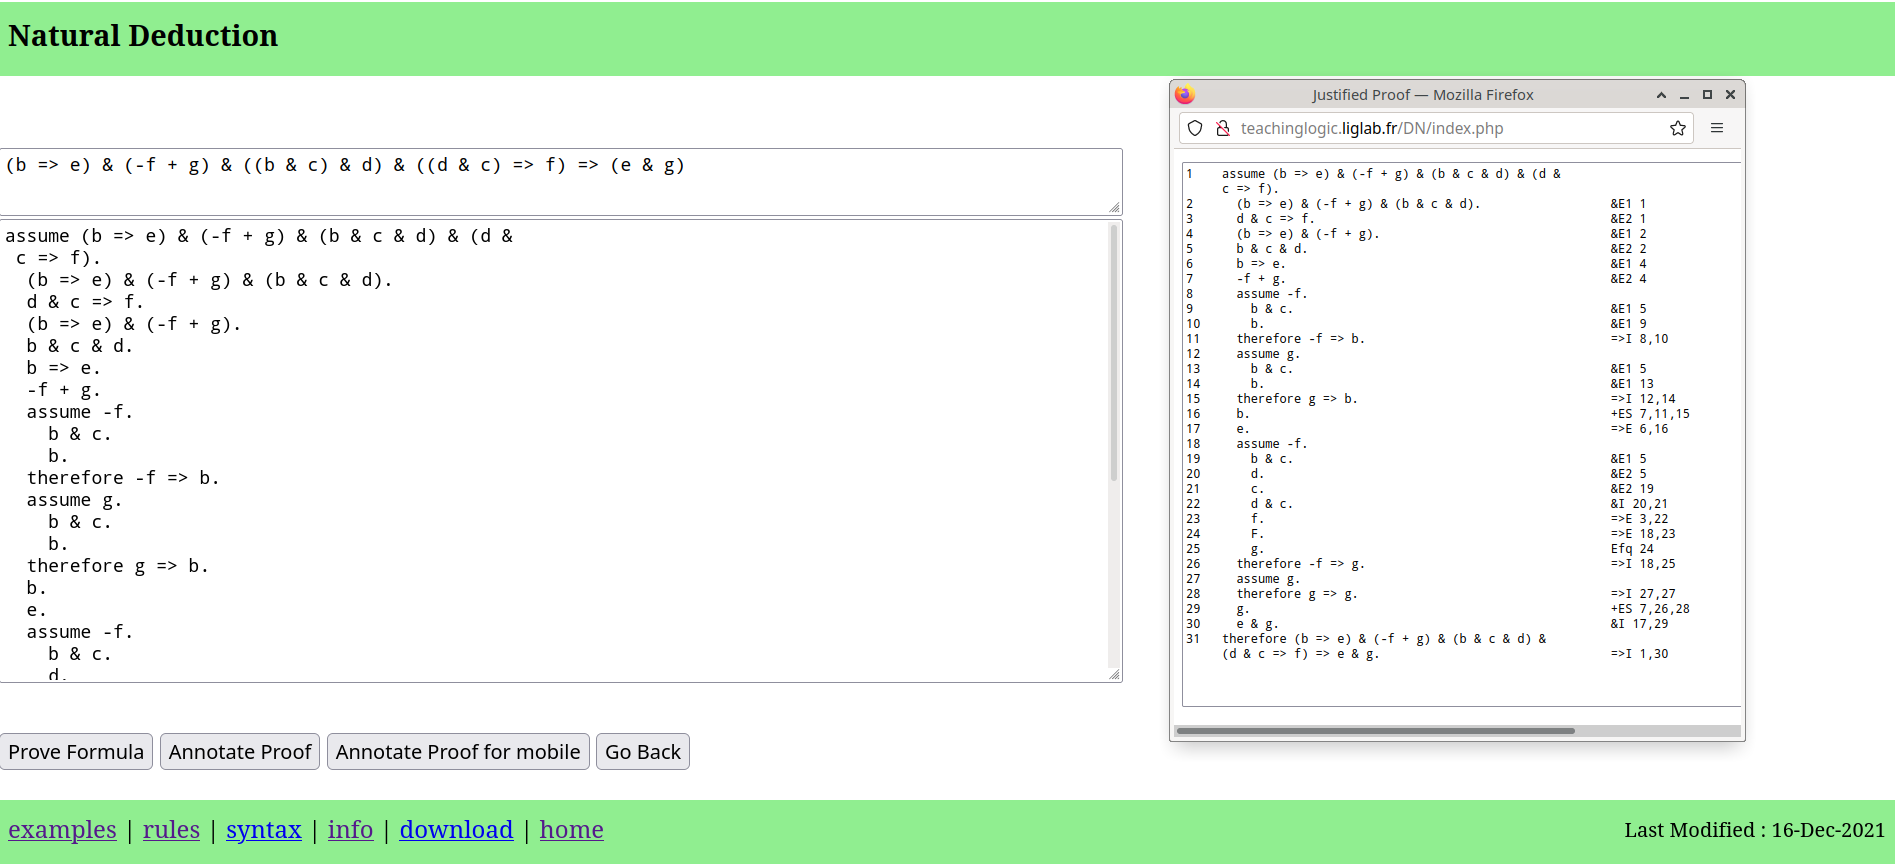
\includegraphics[width=0.65\textwidth]{teachinglogic.png}
        \titlecaption{LIGLAB's Natural Deduction}{Example proof showing the user interface and proof annotations.}
        \label{fig:liglab}
    \end{figure} 
    Natural Deduction is a Windows 10 application designed by Jukka H\"akkinen, and is the second natural deduction software we investigated. This system includes both a proof generator and a proof checker. While it primarily focuses on modal logic (specifically, the modal logic system S5), it has a propositional logic prover because modal logic natural deduction semantics is a superset of propositional logic. We noted that its interface is clean and very elegant to use. Likewise, its ability to prove both theorems and premise-conclusion style proofs is helpful. We also found its performance on par, if not faster than other similar software. However, Natural Deduction has a severe drawback: it's proof generation capabilities, or somewhat of a lack thereof. While it generates short and simple proofs for a subset of our test suite, for others, the proofs were unmanageably long and so cumbersome that a student would, realistically, never look through them. In addition to this significant issue, we discovered that the system places an arbitrary limit on the length of a premise set and its corresponding conclusion. Along a similar vein, the system refuses any proof that contains more than seven propositions/atoms, even if the proof contains no connectives - only atoms (e.g., $A$, $B$, $C$, $D$, $E$, $F$, $G$, $H$, $\therefore$ $H$). Lastly, the system automatically converts connectives to a recognizable format e.g., \textgreater\;to $\to$, and uppercases any entered propositions. It gets confused, though, if the user enters a symbol it does not recognize (e.g., \& instead of $\land$). These restrictions do not entirely detract students from the application; however, they exemplify the types of downfalls that other systems do not have.
    \begin{figure}
        \centering
        \begin{subfigure}{.5\textwidth}
          \centering
          \includegraphics[width=0.9\linewidth]{w10app\_01.png}
          \caption{A subfigure}
          \label{fig:sub1}
        \end{subfigure}%
        \begin{subfigure}{.5\textwidth}
          \centering
          \includegraphics[width=0.9\linewidth]{w10app\_02.png}
          \caption{A subfigure}
          \label{fig:sub2}
        \end{subfigure}
        \caption{A figure with two subfigures}
        \label{fig:test}
    \end{figure}
    \textbf{Now tautlogic}
    TautLogic is...... lorem ipsum  lorem ipsum lorem ipsum lorem ipsum lorem ipsum lorem ipsum lorem ipsum lorem ipsum lorem ipsum lorem ipsum lorem ipsum lorem ipsum lorem ipsum lorem ipsum
    \begin{figure}
        \centering
        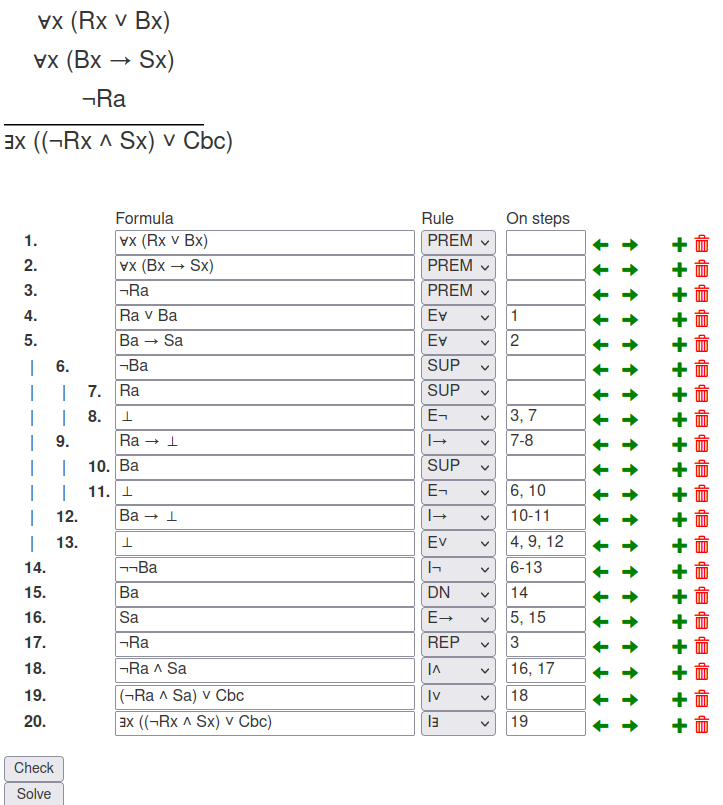
\includegraphics[width=0.65\textwidth]{tautlogic.png}
        \titlecaption{TautLogic's Predicate Natural Deduction}{Write a caption...}
        \label{fig:tautlogic}
    \end{figure} 

    \textbf{Show results of experiment}

    \begin{figure}
        \centering
        \includegraphics[width=0.9\textwidth]{all\_proofs\_graph.png}
        \titlecaption{TautLogic's Predicate Natural Deduction}{Write a caption...}
        \label{fig:allproofsgraph}
    \end{figure} 

    \begin{figure}
        \centering
        \includegraphics[width=0.9\textwidth]{prop\_graph.png}
        \titlecaption{Propositional Logic Natural Deduction}{Write a caption...}
        \label{fig:propgraph}
    \end{figure} 

    \begin{figure}
        \centering
        \includegraphics[width=0.9\textwidth]{pred\_graph.png}
        \titlecaption{Predicate Logic Results Graph}{Write a caption...}
        \label{fig:predgraph}
    \end{figure} 

    \textbf{Discuss challenges with inputting data... which lead to the desire for a gold standard!}    

    \section{Gold Standard for Formal Logic System Syntax}
    There are several reasons why a standardized grammar does not necessarily already exist for formal logic. Firstly, the symbols used vary widely from one subject to the next e.g., notation used in computer science may ave sublte yet important differences from philosophy-esque logics. Secondly, preexisting sources such as textbooks, websites, professors, and others all use preferential notation, leading to an amalgamation of symbols for students to use and reference which, therefore, leads students and automatic systems astray when expecting one syntax yet receive something completely different. Thirdly, propositional logic learning platforms may or may not include certain operators. For example, because it is trivial to represent the biconditional (if and only if) binary operator as a conjunction of implications, it is certainly possible, albeit rather rare, to omit its symbolic representation from a language. Such omissions cause problems when evaluating formulas either automatically or by hand..... \textbf{continue here}

    We propose a formal definition that aims to solve most of these problems. One component of this definition allows users to create their own logic language definition as they see fit for their situation. This language is then translatable into a gold standard format, which we will define syntactically and semantically.

    \subsection{Zeroth-Order Logic Well-Formed Formula Representation}
    Let $M(\mathcal{L},\,w)$ be a function that ``applies'' the zeroth-order logic language $\mathcal{L}$ to the well-formed formula $w$. Let $\mathcal{L}$ be a pair $(f,\,g)$ where $f$ is an connective mapping function, and $g$ is an atomic literal mapping function. 

    The bijective function $f$ maps two sets $f:\;X \to Y$, where $X$ is the set of input connectives defined by $\mathcal{L}$, and $Y \subseteq \{N,\,C,\,D,\,E,\,I,\,B,\,T,\,F\}$ is the set of output connectives defined by our grammar, where $|X| = |Y|$. $N$ is unary logical negation, $C$ is binary logical conjunction, $D$ is binary logical inclusive disjunction, $E$ is binary logical exclusive disjunction, $I$ is binary logical implication, $B$ is binary logical biconditional (if and only if), $T$ is the truth function, and $F$ is the false function. Note that the arity of any $\phi \in X$ must match the arity of its corresponding output connective in $Y$.

    The bijective function $g$ maps two sets $g:\;A \to B$, where $A$ is the set of atomic literals $\psi \in A$ where $\psi$ is an atomic literal used in $w$, and $B$ is the set of output atomic formulas $a_{j}$ where $j \in [1,\,|A|]$.

    We can now define the Polish (Łukasiewicz) notation grammar $G$ used to create a standardized notation for zeroth-order logic. This notation takes inspiration from Scheme-syntax with its parenthesization of connectives and operands. For this, we must extend the definition of typical Extended Backus-Naur Form to account for multiple-arity connectives. Thus, we introduce the notation \textless{$x$---R\textgreater} to indicate that $x$ is a variable used in the EBNF rule $R$, and $\{\gamma\}^{x}$ to denote $x$ applications of $\gamma$. In the grammar, $\alpha$ is the arity of a connective.
    \begin{grammar}
        <atomic> ::= `a' (`1' | `2' | ...)
        
        <connective> ::= `N' | `C' | `D' | `E' | `I' | `B' | `T' | `F' 
        
        <$\alpha$---wff> ::= <atomic> | (<connective> [` '] \{<wff>\}$^{\alpha}$)
    \end{grammar}
    \subsubsection{Example 1.} Let us take a ``standard'' propositional logic language $\mathcal{L}$ and a formula $w$. $\mathcal{L}$ consists of two functions $f$ and $g$ where
    \begin{align*}
        &f:\;\{\supset,\,\land,\,\lor,\,\leftrightarrow,\,\lnot\}\mapsto \{I,\,C,\,D,\,B,\,N\}\\
        &g:\;\{A,\,B,\,C\} \mapsto \{a_{1},\,a_{2},\,a_{3}\}
    \end{align*}
    We will let $w = A \supset (B \leftrightarrow \lnot C)$. Thus, 
    \[
        M(\mathcal{L},\,w) = (I\;a_{1}\;(B\;a_{2}\;(N\;a_{3})))
    \]
    While this representation is not as readable as $w$, it creates a uniform standard for testing zeroth-order logic systems. What's more is that this application process is reversible; given $M^{-1}(\mathcal{L}',\,w')$ where $\mathcal{L}' = (f^{-1},\,g^{-1})$ and $w' = M(\mathcal{L},\,w)$, we can reproduce $w$ using a simple stack-and-pop parsing evaluation approach (deterministic push-down automaton).
    
    The reason we formalize the language definition is to allow different logic systems with varying syntax---some use lower-case atomic formulas, while others may restrict the alphabet to a subset. This definition allows different connective alphabets to map to the same symbol in the gold standard which provides a seamless translation to and from various host logic languages (i.e., the language of the implementing systems, assuming it does not, by default, use the gold standard internally).

    \subsubsection{Natural Deduction Extension.} It is simple to extend $G$ to support premises and conclusions using the same syntax. We can define a new function $N(\mathcal{L},\,P,\,c)$, where $\mathcal{L}$ is the same definition as before, $P$ is a set of well-formed formula acting as the premises of the proof, and $c$ is the well-formed formula acting as the conclusion of the proof. Our new grammar $G'$ is as follows:

\begin{grammar}
<atomic> ::= `a' (`1' | `2' | ...)

<connective> ::= `N' | `C' | `D' | `E' | `I' | `B' | `T' | `F' 

<$\alpha$---wff> ::= <atomic> | (<connective> [` '] \{<wff>\}$^{\alpha}$)

<premise> ::= (`P' <wff>)

<conclusion> ::= (`H' <wff>)

<proof> ::= (<conclusion> \{<premise>\})
\end{grammar}

The preceding grammar states that a premise is preceded by the letter $P$ standing for \textit{premise}, conclusions are preceded by $H$ for \textit{hence}, and a proof is a conclusion followed by zero or more premises (a proof with zero premises is a theorem).\\

%~(C ∨ D), D ↔ (E ∨ F), ~A → (C ∨ F) ∴ A
\subsubsection{Example 2.}
Let's create a proof where $P = \{\lnot(C \lor D),\,D \leftrightarrow (E \lor F), \lnot A \supset (C \lor F)\}$, and $c = A$. We must redefine the function $g$ in $\mathcal{L}$ as follows:
\[
    g:\;\{A, C, D, E, F\} \mapsto \{a_1,\,a_2,\,a_3,\,a_4,\,a_5\}
\]
\noindent Thus, 
\begin{align*}
    N(\mathcal{L}, P, c) &= ((H\;a_1)\;\\
    &(P\;(N\;(D\;a_2\;a_3)))\\
    &(P\;(B\;a_3\;(D\;a_4\;a_5)))\\
    &(P\;(I\;(N\;a_1)\;(D\;a_2\;a_5))))\\
\end{align*}
\subsection{First-Order Logic Well-Formed Formula Representation}

First-order logic is a superset of zeroth-order logic, meaning we can reuse most of our definitions from the previous section. We will, however, need to slightly redefine $\mathcal{L}$ to allow for mapping predicate definitions, constants, and variables. Further, so as to not confuse the function definitions from zeroth-order logic, we will instead use new letters to represent mapping functions.

Let $\mathcal{L}$ be a quadruple $(p,\;q,\;r,\;s)$ where $p$ is a connective mapping function, $q$ is a predicate mapping function, $r$ is a constant mapping function, and $s$ is a variable mapping function. 

The bijective function $p$ is identical to $f$ in the sense that it maps two sets $p:\;X \to Y$, where $X$ is the set of input connectives defined by $\mathcal{L}$, and $Y \subseteq \{N, C, D, E, I, B, T, F, Z, X, V\}$ is the set of output connectives defined by our grammar, where $|X| = |Y|$. $N$, $C$, $D$, $E$, $I$, $B$, $T$, and $F$ are identical in both syntactic and semantic meaning to zeroth-order logic. $Z$ is the universal quantifier, $X$ is the existential quantifier, and $V$ is the identity operator. $Z$ and $X$ have arities dependent on the formula used, so we cannot restrict it syntactically. Identity $V$, on the other hand, is a binary operator.

The bijective function $q$ maps two sets $q:\;A \to B$, where $A$ is the set of predicate letters $\phi \in A$ where $\phi$ is a predicate letter used in the wff $w$, and $B$ is the set of output predicate letters $L_{i}$ where $i \in [1, |A|]$.

The bijective function $r$ maps two sets $r:\;C \to D$, where $C$ is the set of constant letters $\psi \in C$ where $\psi$ is a constant identifier used in $w$, and $D$ is the set of output constant identifiers $c_{i}$ where $i \in [1, |C|]$.

Lastly, the bijective function $s$ maps two sets $s:\;E \to F$, where $E$ is the set of variable letters $\rho \in E$ where $\rho$ is a variable identifier used in $w$ and $F$ is the set of output variable identifiers $v_{i}$ where $i \in [1, |E|]$.

Now, similar to zeroth-order logic, we will construct the gold standard Polish notation grammar $H$ for first-order logic. Likewise, we will utilize the previously-defined notation \textless{$x$---R\textgreater} to eliminate ambiguity with operator arity. One point to note is that, because identity is a special connective in first-order logic, we restrict its syntactic definition to only constants and variables. Quantifiers also have a restriction in that they must have at least one variable following their declaration, as well as a bound well-formed formula.
\begin{grammar}

    <constant> ::= `c' (`1' | `2' | ...)

    <variable> ::= `v' (`1' | `2' | ...)

    <literal> ::= <constant> | <variable>

    <predicate> ::= `L' (`1' | `2' | ...)

    <connective> ::= `N' | `C' | `D' | `E' | `I' | `B' | `T' | `F'

    <identity> ::= `V'

    <quantifier> ::= `Z' | `X'

    <$\alpha$---wff> ::= (<predicate> \{<literal>\}) \\| (<connective> [` '] <wff>$^{\alpha}$) \\| (<quantifier> <variable> \{<variable>\} <wff>)\\| (<identity> <literal> [` '] <literal>)
\end{grammar}

The above grammar states ...\textbf{continue here}
\subsubsection{Example 3.} We will, once again, use a ``standard'' first-order logic language $\mathcal{L}$ and a formula $w$. $\mathcal{L}$ consists of the four functions $p$, $q$, $r$, and $s$ where
\begin{align*}
    &p:\;\{\supset,\,\land,\,\lor,\,\leftrightarrow,\,\lnot,\,\forall,\,\exists,\,=\}\mapsto \{I,\,C,\,D,\,B,\,N,\,Z,\,X,\,V\}\\
    &q:\;\{P,\,Q,\,R\} \mapsto \{L_{1},\,L_{2},\,L_{3}\}\\
    &r:\;\{c,\,d\} \mapsto \{c_1,\,c_2\}\\
    &s:\;\{x,\,y,\,z\} \mapsto \{v_1,\,v_2,\,v_3\}
\end{align*}
Suppose $w = \forall{x}\forall{y}\lnot{Pxyc} \land (Qcd \lor \exists{z}Rz)$. Thus,
\begin{align*}
    M(\mathcal{L},\,w) &= (C\;(Z\;v_1\;(Z\;v_2\;(N\;(L_1\;v_1\;v_2\;c_1))))\\
    &(D\;(L_2\;c_1\;c_2)\;(X\;v_3\;(L_3\;v_3))))\\
\end{align*}

\chapter{Discussion and Future Direction}


\bibliographystyle{acm}
\bibliography{myreferences}
\nocite{*}

%%------------------------------------------------------------------%%
%%------------------------- Appendices -----------------------------%%
%%------------------------------------------------------------------%%
%% If you choose not to have appendices, comment out the \appendix
%% line and the chapters below.
%%------------------------------------------------------------------%%
\appendix
\chapter{Propositional Logic Natural Deduction Algorithm}

This appendix describes the algorithm we used to find a natural deduction proof for propositional logic. The idea is to use a ``satisfiability'' algorithm. A wff $w$ is satisfied when it is used in the reduction or expansion of another well-formed formula $w'$. In essence, if $w$ is used to construct $w'$, then $w$ is satisfied. At a high level, we recursively compute goals for each premise, and if we can satisfy each goal, then the premise is satisfied. The procedure \textsc{Satisfy} uses rules for each axiom to determine if a premise can be either simplified or if, as a goal, it can be constructed using other premises. For example, suppose we have two premises $A$ and $B$ and we want to satisfy $A \land B$. \textsc{Satisfy} will recursively search through the well-formed formula (i.e., search the left and right operands) to determine if either have been previously satisfied. Given that $A$ and $B$ are already premises, and premises are, by default, satisfied, we can conlude that $A \land B$ is satisfiable. As another example, let us take the argument $P = \{A \supset (B \land \lnot C),\;\lnot (B \land \lnot C)\}$ and $c = \lnot A$. It is trivial to see t hat we can conclude $c$ from the premises in $P$ via a modus tollens rule. \textsc{Satisfy} works slightly different when this type of situation occurs. Because all premises are satisfied by default, and there is no way to individually solve intermediate formulas e.g., $B$, $\lnot C$, the algorithm searches for transformations and elimination rules e.g., modus ponens, modus tollens, disjunctive syllogism, transposition, material implication, etc., that may be applied to premises. In our provided example, we can apply modus tollens to the two premises and consequently satisfy $\lnot{A}$. $\lnot{A}$ is, therefore, added to $P$. The terminating condition is when $c$ is satisfied, or $c \in P$. Because there are numerous transformations that may be applied to premises, we will omit their direct inclusion in favor of a broad description of behaviors. To prevent unnecessary premises, once a premise is satisfied, it can never be ``unsatisfied''. Moreover, if a premise was constructed, it cannot be redundantly destructed or vice versa. For instance, suppose we have premises $A$ and $B$. We can use a conjunction introduction $\land{I}$ rule to satisfy $(A \land B)$. The algorithm could, in theory, use a conjunction elimination $\land{E}$ rule to break $(A \land B)$ back down into its original components. Since such an application blows up the size of $P$ (leading to a potentially infinitely long proof), we heuristically prevent its occurrence.

\begin{algorithm}
    \caption{Propositional Natural Deduction Satisfaction Algorithm}\label{euclid}
    \begin{algorithmic}[1]
      \Procedure{Prove}{$P,\;c$}\Comment{$P$ is a list of premises, $c$ is conclusion}
        \While{$c$ is not satisfied}
            \For{$i\gets{1}$ to $P$.length}
                \If{\textsc{Satisfy}($P[i]$)}
                    \State $P[i].satisfied\gets{\textbf{true}}$
                \EndIf
            \EndFor
            \If{\textsc{Satisfy($c$)}}
                \State $c.satisfied\gets{\textbf{true}}$
            \EndIf
        \EndWhile
      \EndProcedure
    \end{algorithmic}
  \end{algorithm}

\backmatter
\end{document}
